S'han assolit tots els requisits i tasques establertes pel projecte. El motor resultant actualment té el nom provisional de Z5, en referència a la saga de videojocs 4X espacials anomenats X, publicada pel desenvolupador Egosoft.
El motor està publicat sota llicència GPL3 a \href{https://github.com/theKlanc/Z5}{Github}. A més de les plataformes inicials, també es pot compilar per a Windows utilitzant Visual Studio, i també per web utilitzant emscripten.
Els binaris estàn disponibles sota la secció de Releases al repositori de Github, i una build experimental de la versió emscripten està disponible a \url{http://z5.ledgedash.com/}, però el suport dels navegadors és limitat i pot no funcionar.

\section{Captures de pantalla}
\begin{figure}[]
  \centering
  \includegraphics[scale=0.1]{fotoSwitch}
  \caption{Fotografía de la demo executant-se en una Nintendo Switch.}
\end{figure}
\begin{figure}[]
  \centering
  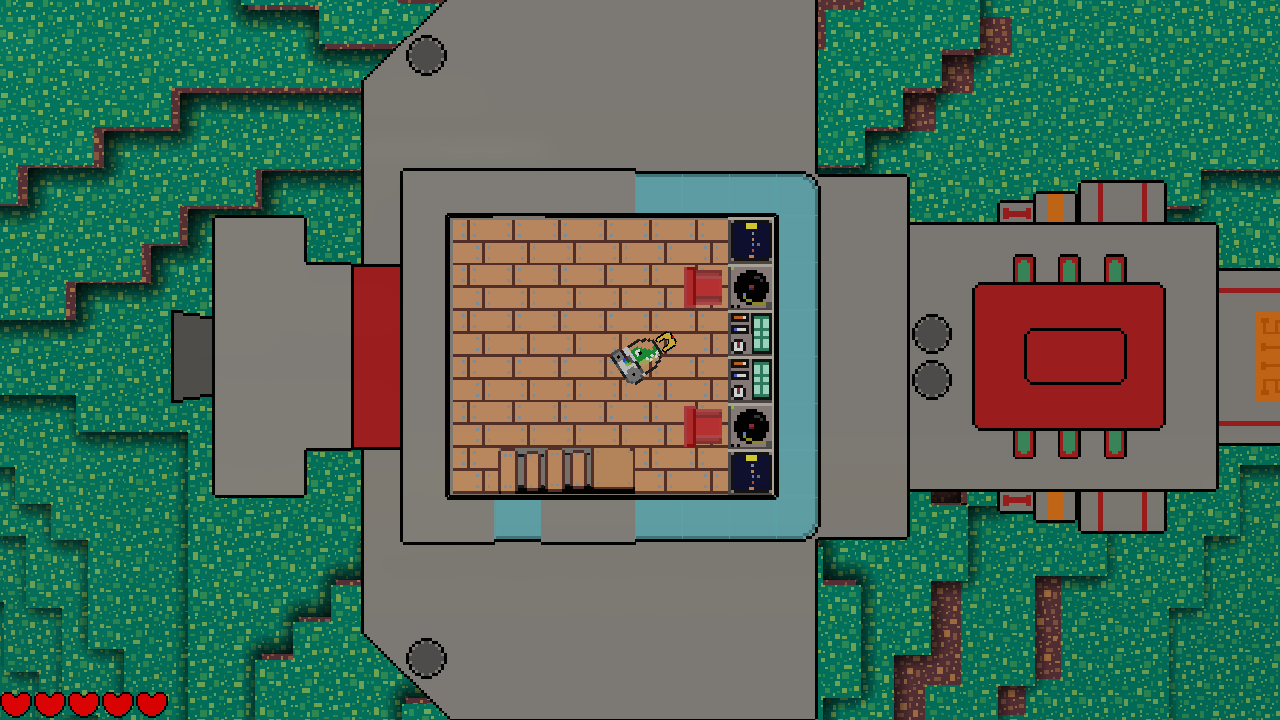
\includegraphics[scale=0.4]{game2}
  \caption{Captura de la demo amb el jugador dins la nau Roc.}
\end{figure}
\begin{figure}[]
  \centering
  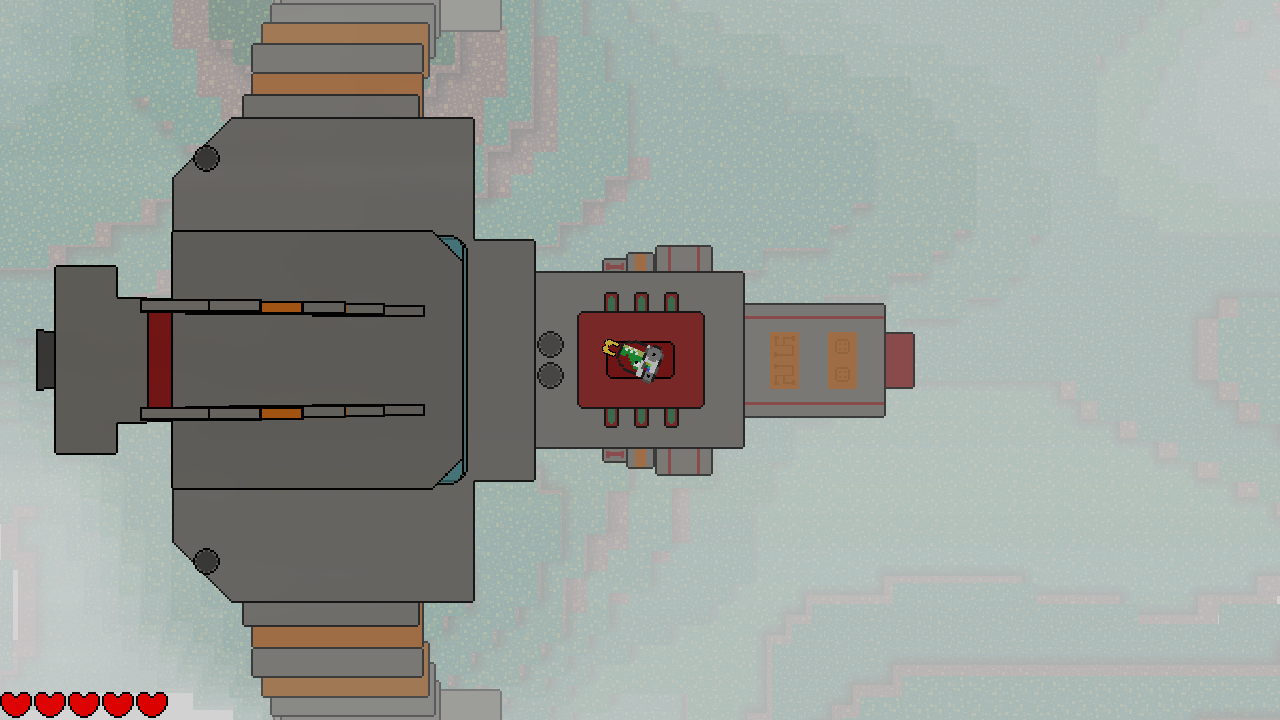
\includegraphics[scale=0.4]{game1}
  \caption{Captura de la demo amb el jugador fora la nau.}
\end{figure}
\begin{figure}[]
  \centering
  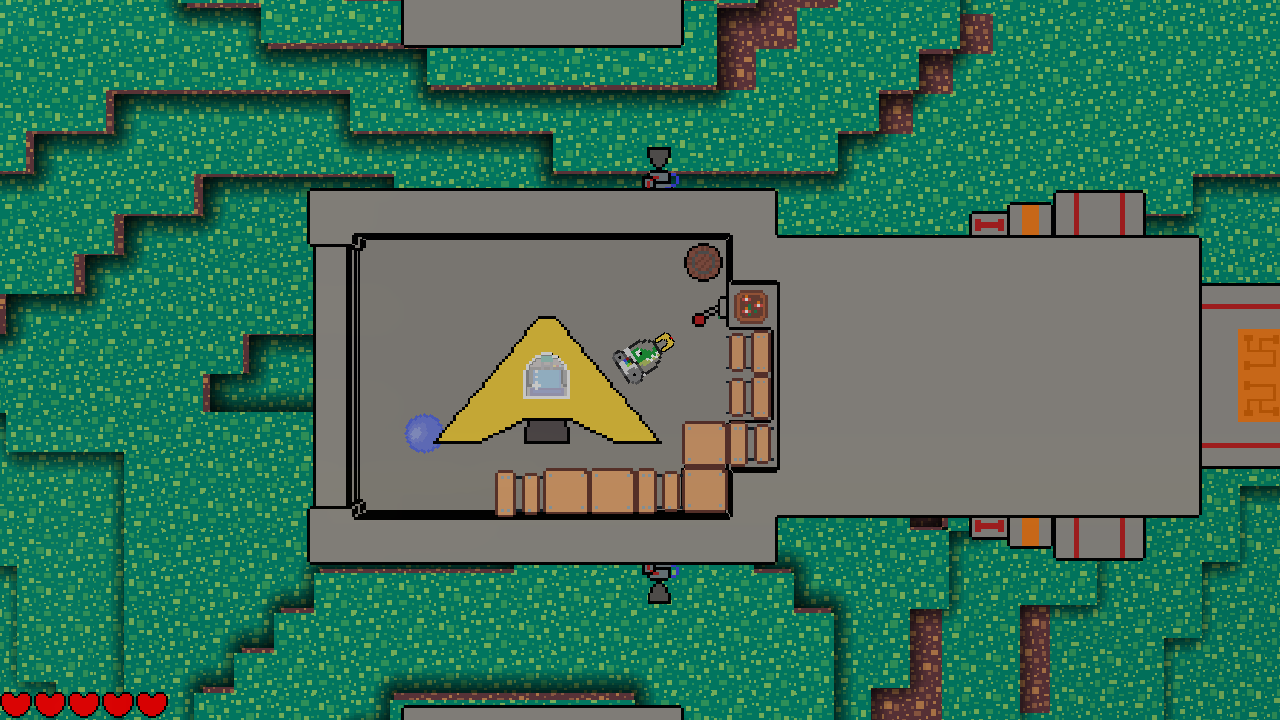
\includegraphics[scale=0.4]{game3}
  \caption{Captura de la demo amb el jugador fins l'hangar de la nau.}
\end{figure}
\begin{figure}[]
  \centering
  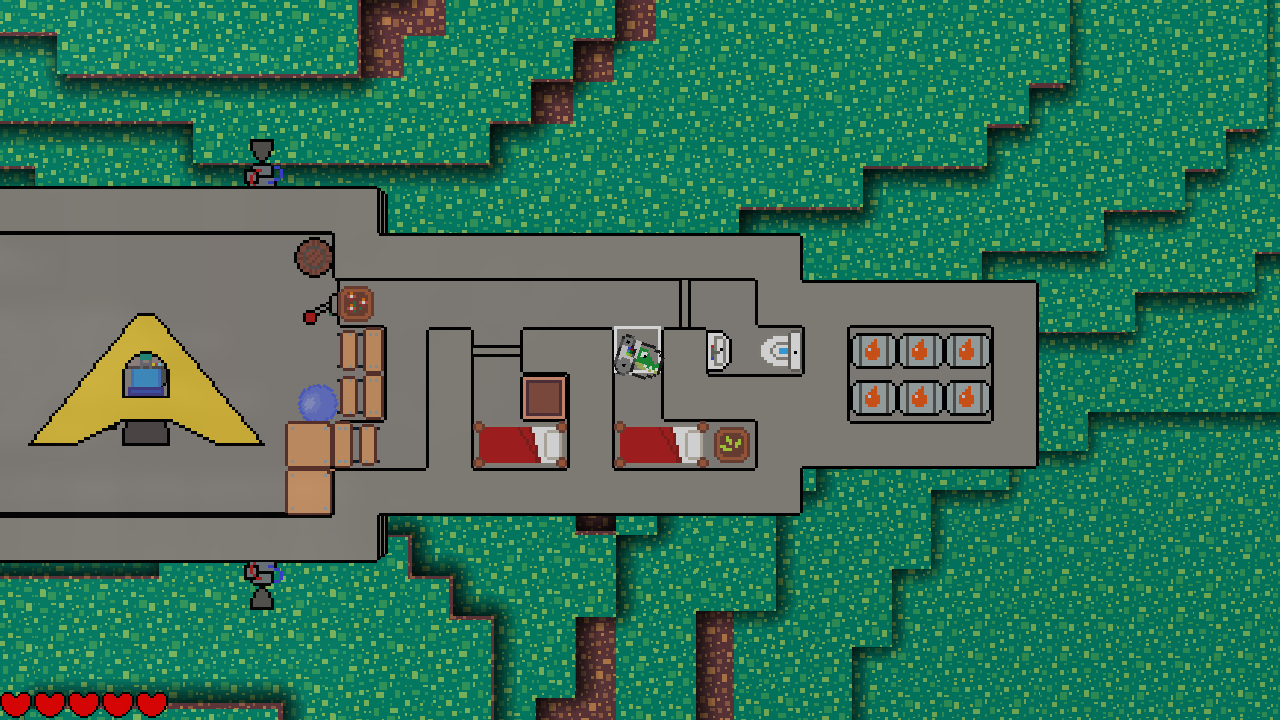
\includegraphics[scale=0.4]{game4}
  \caption{Captura de la demo amb el jugador dins una habitació.}
\end{figure}
\begin{figure}[]
  \centering
  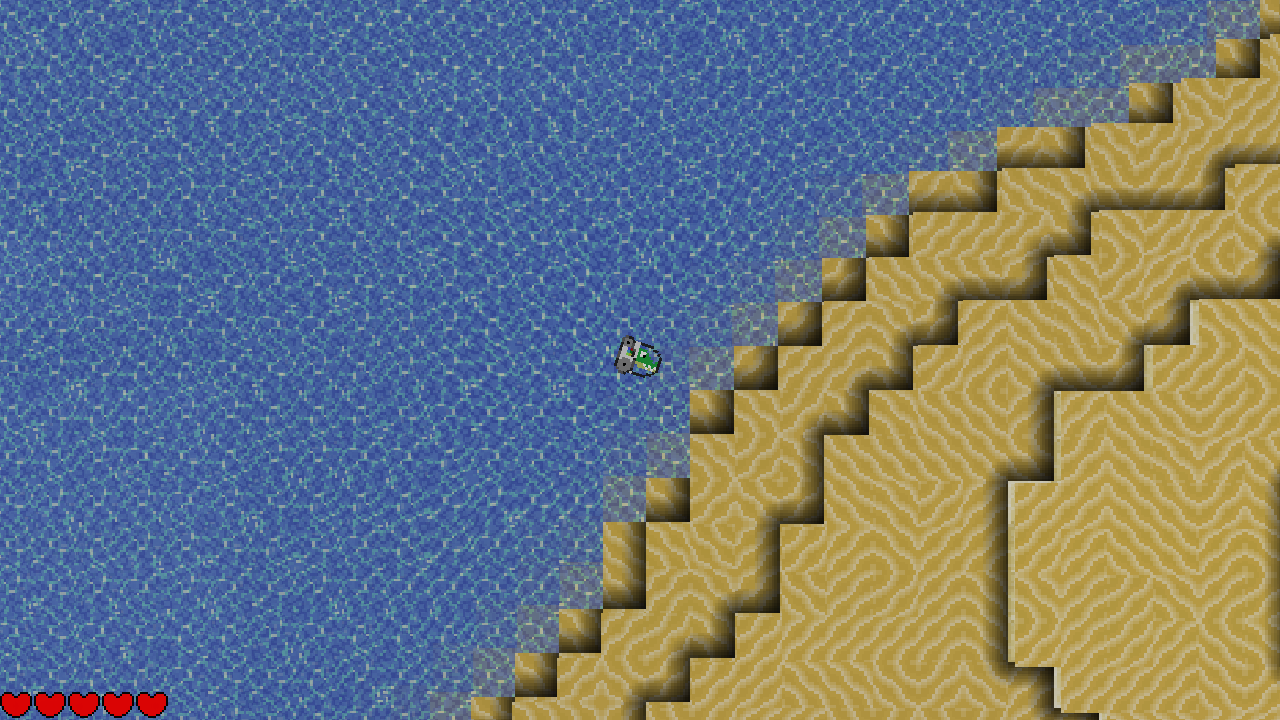
\includegraphics[scale=0.4]{game5}
  \caption{Captura de la demo amb el jugador nedant a la costa.}
\end{figure}
\begin{figure}[]
  \centering
  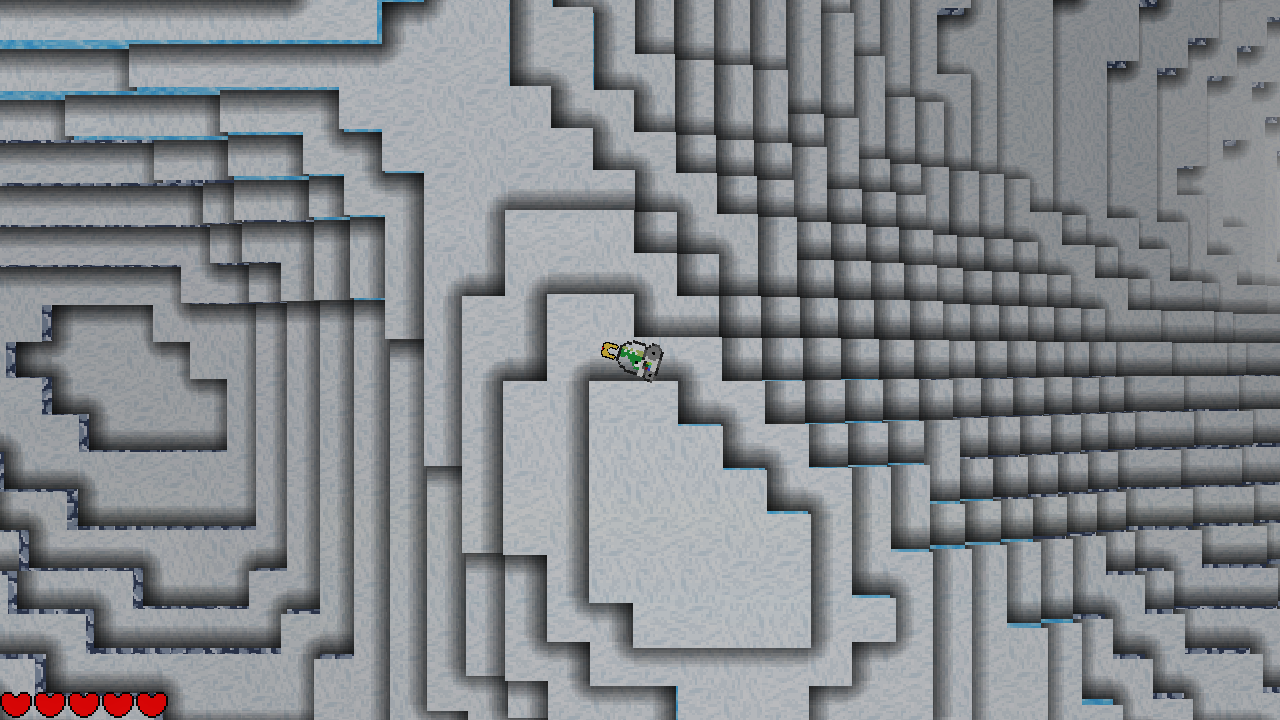
\includegraphics[scale=0.4]{game6}
  \caption{Captura de la demo amb el jugador en una regió muntanyosa nevada.}
\end{figure}
\begin{figure}[]
  \centering
  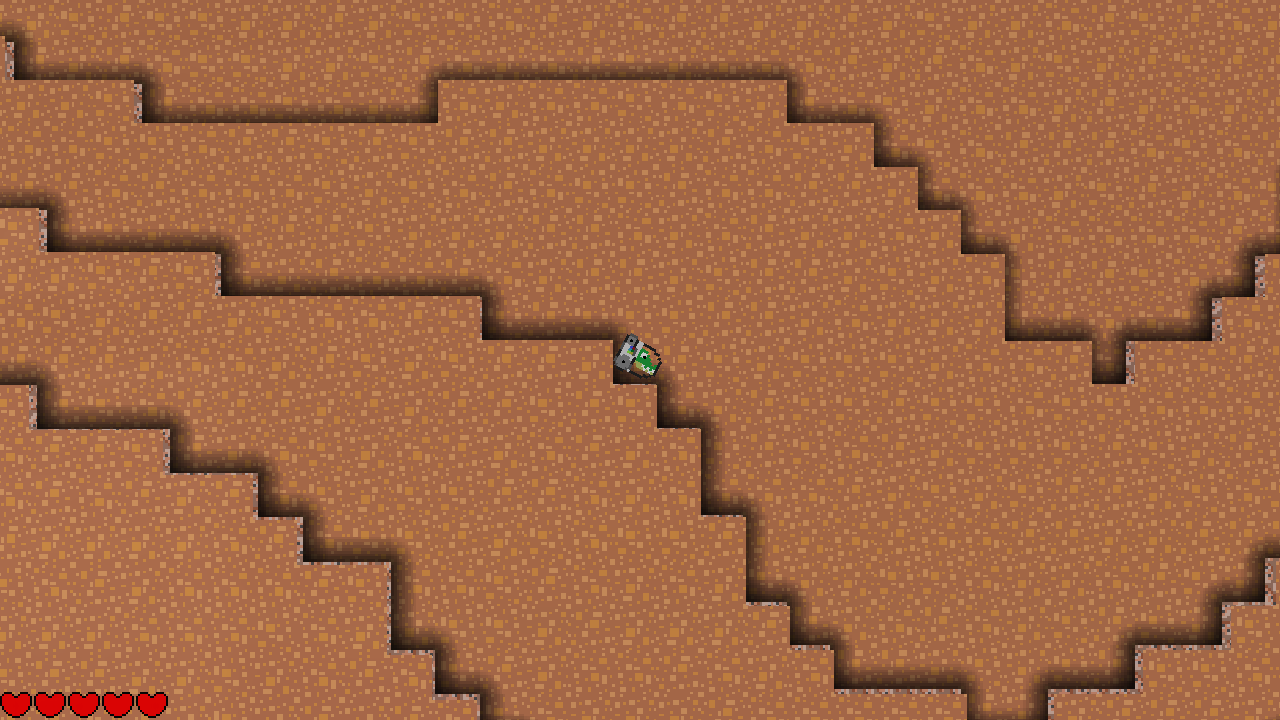
\includegraphics[scale=0.4]{game7}
  \caption{Captura de la demo amb el jugador a la superfície de Mart.}
\end{figure}
\begin{figure}[]
  \centering
  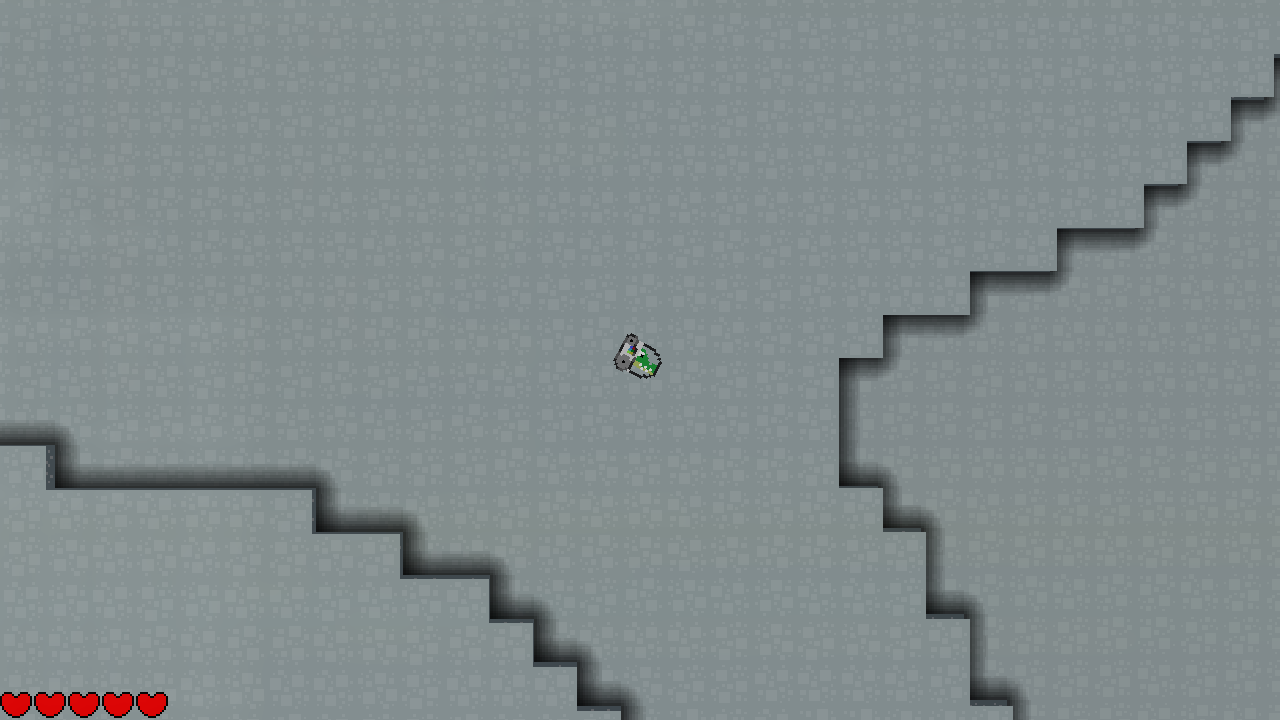
\includegraphics[scale=0.4]{game8}
  \caption{Captura de la demo amb el jugador a la superfície de la Lluna.}
\end{figure}
\begin{figure}[]
  \centering
  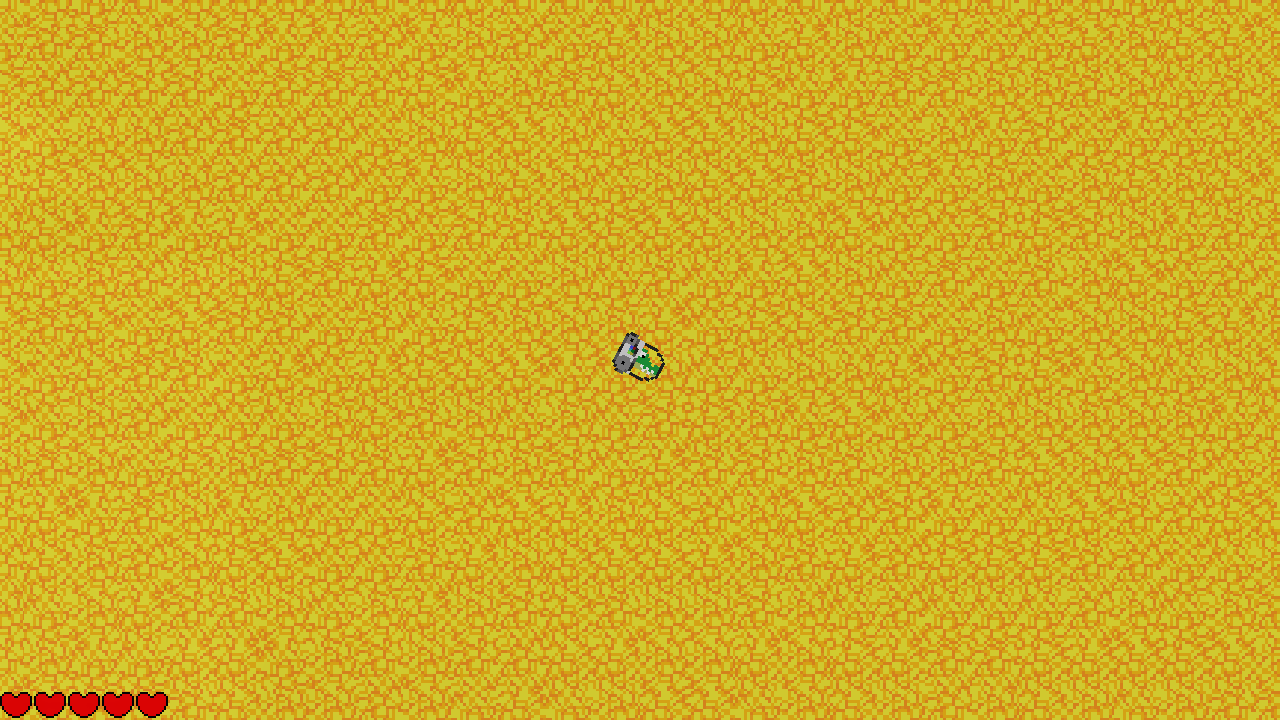
\includegraphics[scale=0.4]{game9}
  \caption{Captura de la demo amb el jugador dins del Sol.}
\end{figure}
\begin{figure}[]
  \centering
  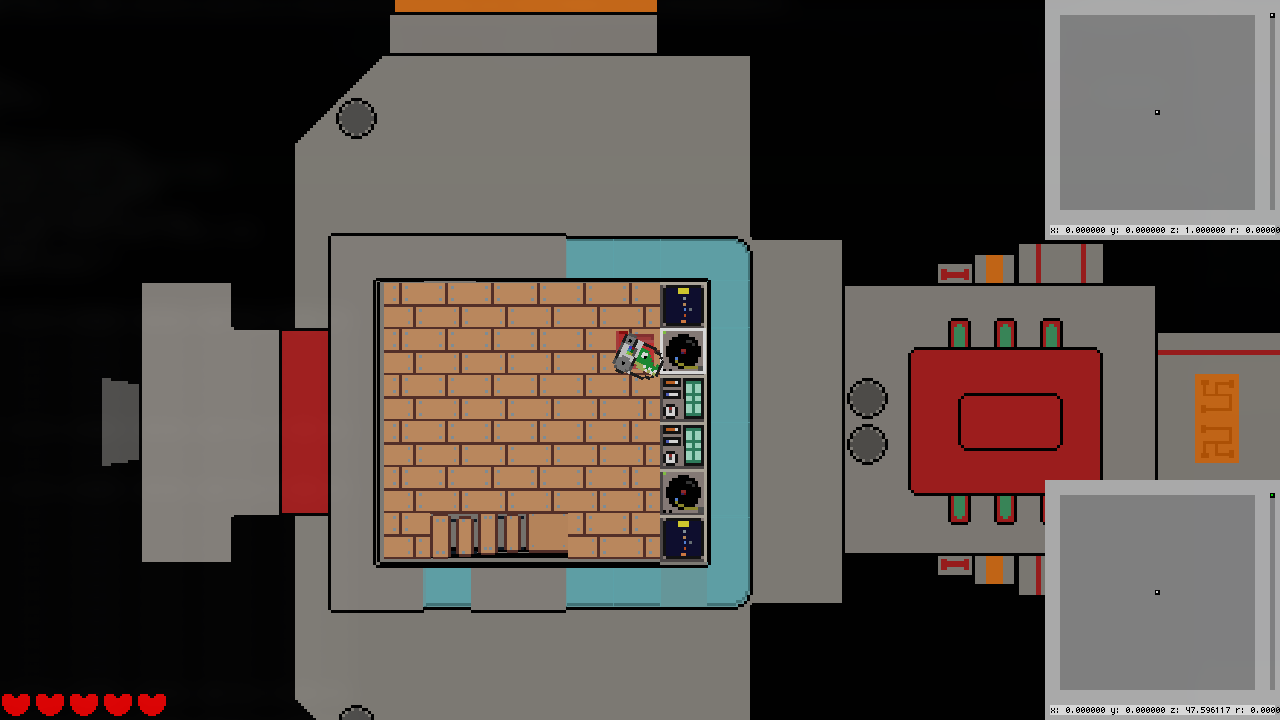
\includegraphics[scale=0.4]{game10}
  \caption{Captura de la demo amb el jugador pilotant la nau per l'espai.}
\end{figure}
\begin{figure}[]
  \centering
  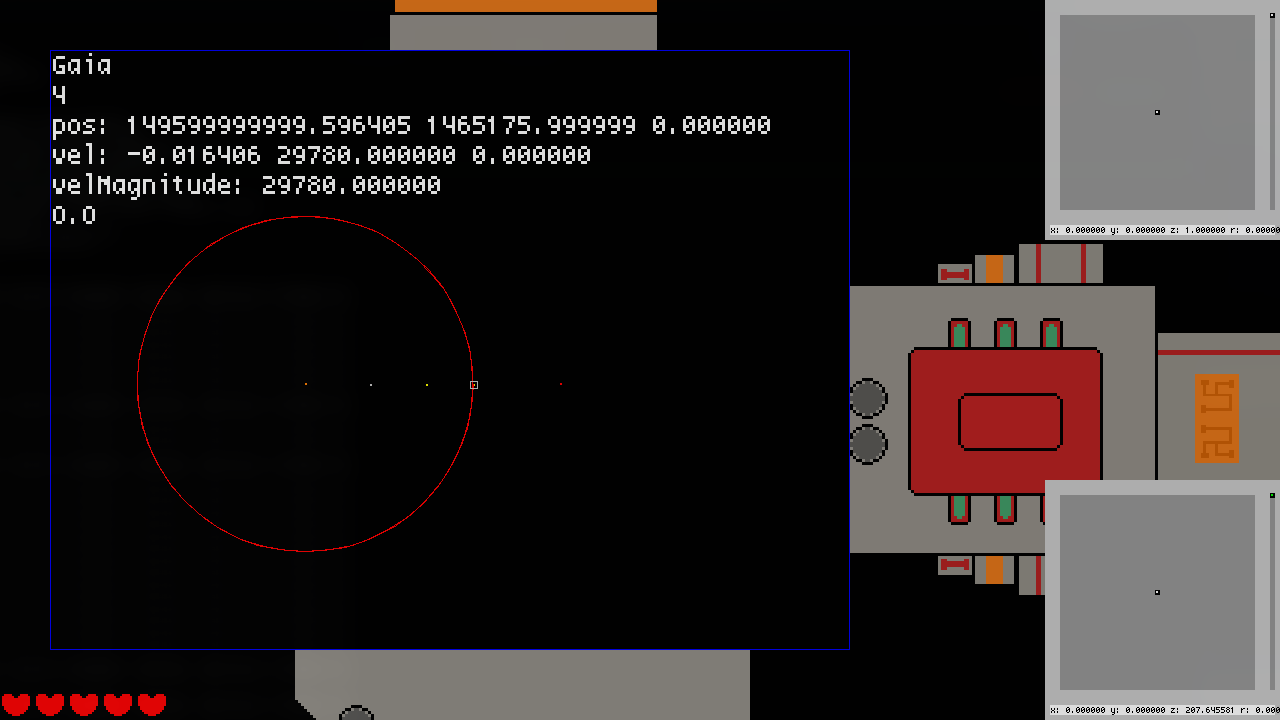
\includegraphics[scale=0.4]{game11}
  \caption{Captura de la demo amb el mapa estelar desplegat, mostrant l'òrbita de la Terra al voltant del Sol.}
\end{figure}
\begin{figure}[]
  \centering
  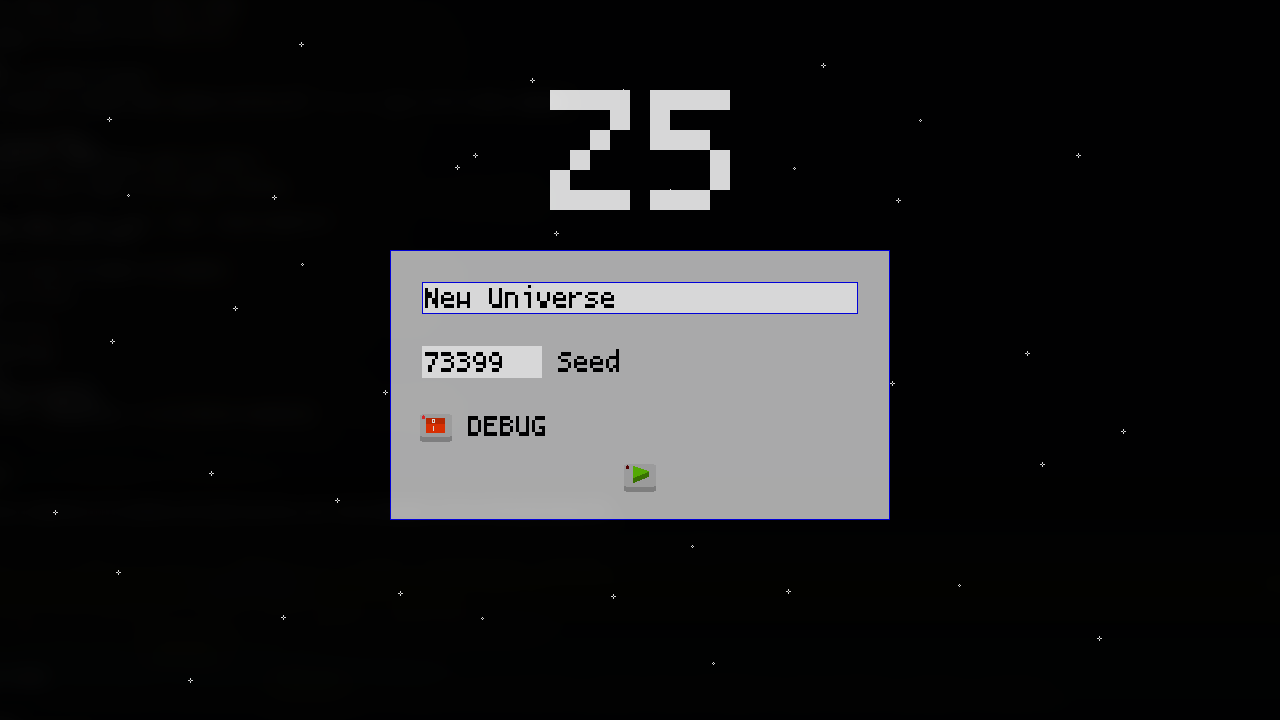
\includegraphics[scale=0.4]{newGame}
  \caption{Captura del menú de creació de partida nova.}
\end{figure}
\begin{figure}[]
  \centering
  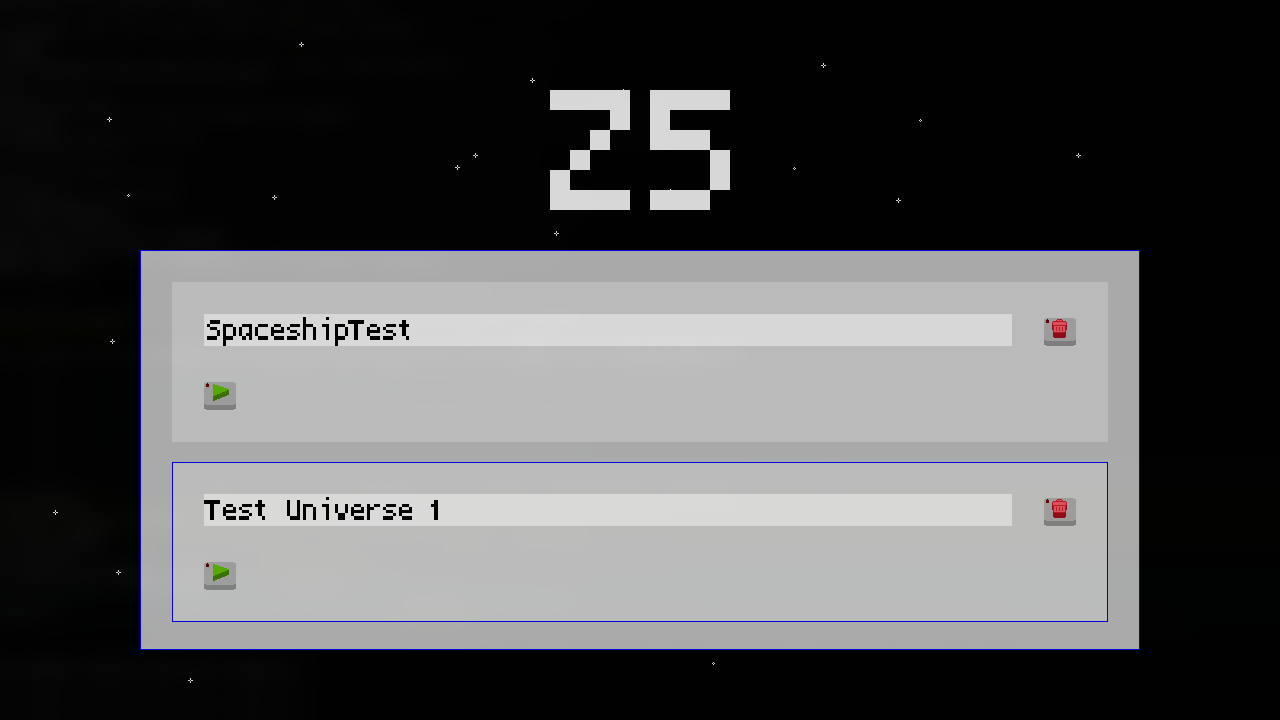
\includegraphics[scale=0.4]{gameSelect}
  \caption{Captura del menú de selecció de partida.}
\end{figure}
\begin{figure}[]
  \centering
  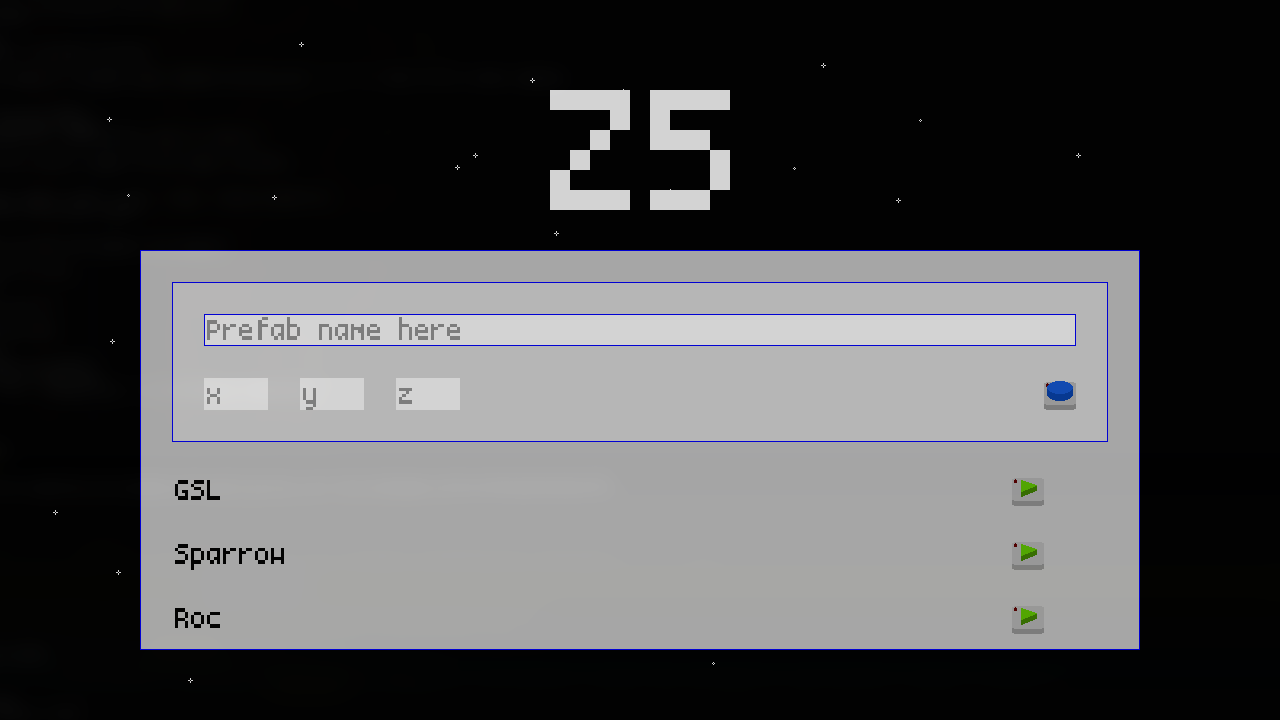
\includegraphics[scale=0.4]{prefabMenu}
  \caption{Captura del menú d'edicio de prefabs.}
\end{figure}
